\documentclass[a4paper,12pt]{article}
\usepackage{graphicx, float, enumerate, parskip}
%\usepackage[indonesian]{babel}
\usepackage{amsmath, amsthm, amssymb, amsfonts}
\theoremstyle{definition}
\newtheorem{definition}{Definisi}[section]
\newtheorem{theorem}{Teorema}[section]
\newtheorem{example}{Contoh}[section]
\usepackage{listings, fancyvrb, spverbatim, xcolor}
\lstset{% setup listings
    language=R,% set programming language
    frame=tb,
    basicstyle=\ttfamily\small,% basic font style
    keywordstyle=\color{blue},% keyword style
    commentstyle=\color{gray},% comment style
    breaklines=true,% automatic line breaking
    fancyvrb=true,% verbatim code is typset by listings
}
\usepackage[
    backend=biber,
    style=bwl-FU,
    sorting=nyt,
    maxbibnames=99,
    natbib=true,
]
{biblatex}
\addbibresource{DPustaka.bib}
\usepackage[
    pdfusetitle,
    colorlinks=true,
    linktoc=page,
    allcolors=blue
]{hyperref}

%% ---------------------------
\begin{document}
    \title{Bootstrap dan Jackknife}
    \author{Addin Zaidan Zakki 4112321026\\
    Fadilatul Husna 4112321032\\
    }
\date{\today}
\begin{titlepage}
    \maketitle
\end{titlepage}

\section{Metode Bootstrap}
Metode Bootstrap adalah kelas metode Monte Carlo nonparametrik yang mengestimasi distribusi populasi dengan resampling. Metode pengambilan sampel ulang memperlakukan sampel yang diamati sebagai populasi terbatas, dan sampel acakdihasilkan (sampel ulang) darinya untuk memperkirakan karakteristik populasi dan membuatnya kesimpulan tentang populasi sampel. Metode bootstrap sering digunakan ketika distribusi populasi sasaran tidak ditentukan; sampel adalahsatu-satunya informasi yang tersedia.

Istilah "bootstrap" dapat merujuk pada bootstrap nonparametrik atau parametrik bootstrap. Metode Monte Carlo yang melibatkan pengambilan sampel dari yang ditentukan sepenuhnya distribusi probabilitas, seperti metode Bab 7 terkadang disebut bootstrap parametrik. Bootstrap nonparametrik adalah pokok bahasan bab ini.
Dalam bootstrap nonparametrik, distribusi tidak ditentukan.

Distribusi populasi hingga yang diwakili oleh sampel dapat
dianggap sebagai populasi semu dengan karakteristik yang mirip dengan populasi sebenarnya. Dengan berulang kali menghasilkan sampel acak dari populasi semu ini (resampling), distribusi sampling dari suatu statistik dapat diperkirakan. Sifat-sifat estimator seperti bias atau standard error dapat diestimasi dengan pengambilan sampel ulang.

Estimasi bootstrap dari distribusi sampling analog dengan ide tersebut estimasi kepadatan. Kami membangun histogram sampel untuk mendapatkan perkiraan bentuk fungsi kerapatan. Histogram bukanlah kepadatan,tetapi dalam masalah nonparametrik, dapat dilihat sebagai perkiraan yang masuk akal
kepadatan. Kami memiliki metode untuk menghasilkan sampel acak sepenuhnya kepadatan tertentu; bootstrap menghasilkan sampel acak dari empiris distribusi sampel

\subsection{Estimasi Bootstrap dari Standard Error}
Estimasi bootstrap dari kesalahan standar estimator $\widehat{\theta }$ adalah sampelnya deviasi standar dari replikasi bootstrap $\widehat{\theta }^{\left ( 1 \right )},,,,,$




\begin{equation}
    \widehat{se}\left ( \widehat{\theta ^{*}} \right )=\sqrt{\frac{1}{B-1}\sum_{b=1}^{B}\left ( \widehat{\theta } ^{\left ( b \right )}-\overline{\widehat{\theta^{*} }}\right )^{2}}y
\end{equation}
dimana $\overline{\widehat{\theta ^{*}}}=\frac{1}{B}\sum_{b=1}^{B}\widehat{\theta}^{(b)}\left [ 91,(6,6) \right ]$

\begin{example}
    (Estimasi Bootstrap dari kesalahan standar). Data sekolah hukum
mengatur hukum di paket bootstrap [286] berasal dari Efron dan Tibshirani [91]. Itu
bingkai data berisi LSAT (skor rata-rata pada skor ujian masuk sekolah hukum)
dan IPK (rata-rata nilai rata-rata sarjana) untuk 15 fakultas hukum.

    LSAT 576 635 558 578 666 580 555 661 651 605 653 575 545 572 594
    
    GPA  339 330 281 303 344 307 300 343 336 313 312 274 276 288 296

    Kumpulan data ini adalah sampel acak dari 82 sekolah hukum di dunia hukum82
(bootstrap). Perkirakan korelasi antara skor LSAT dan IPK, dan
hitung estimasi bootstrap dari kesalahan standar dari korelasi sampel.
\begin{enumerate}
    \item Untuk setiap replikasi bootstrap, di indeks b = 1, . . . , B:
    
        (a) Hasilkan sampel $x^{^{a}(b)}=x_{1}^{*},.....,x_{n}^{*}$ dengan  
        pengambilan sampel dengan penggantian dari sampel yang diamati $x_{1},.....,x_{n}$

        (b) Hitung $b^{th}$ mengulangi $\hat{\theta ^{(b)}}$ dari $b^{th}$ 
        sampel bootstrap, dimana $\hat{\theta ^{(b)}}$ adalah sampel korelasi R antara (LSAT, GPA).
    \item Estimasi bootstrap dari se(R) adalah standar deviasi sampel dari
       ulangan $\hat{\theta ^{(1)}}$,......,$\hat{\theta^{(B)}}=R^{(1)},......,R^{B}$
\end{enumerate}
   
\begin{lstlisting}
    library(bootstrap) #for the law data
    print(cor(law$LSAT, law$GPA))
    [1] 0.7763745
    print(cor(law82$LSAT, law82$GPA))
    [1] 0.7599979
\end{lstlisting}
    Korelasi sampel R = 0,7763745. Korelasi untuk alam semesta dari 82 sekolah hukum R = 0,7599979. Gunakan bootstrap untuk memperkirakan kesalahan standar dari statistik korelasi dihitung dari sampel nilai dalam hukum.
\begin{lstlisting}
    #menyiapkan bootstrap
    B <- 200               #jumlah ulangan
    n <- nrow(law)         #ukuran sampel
    R <- numeric(B)        #penyimpanan untuk ulangan

   #estimasi bootstrap dari kesalahan standar R
   untuk (b dalam 1:B) {
        #pilih indeks secara acak
        i <- sampel(1:n, size = n, replace = TRUE)
        LSAT <- law$LSAT[i]         #i adalah vektor indeks
        GPA <- law$GPA[i]
        R[b] <- cor(LSAT, GPA)
    }
    #output
    #output
    > print(se.R <- sd(R))
    [1] 0.1358393
    > hist(R, prob = TRUE)
\end{lstlisting}
Estimasi bootstrap se(R) adalah 0,1358393. Perkiraan teori normal untuk standard error R adalah 0,115. Metode jackknife-after-bootstrap untuk menghitung waktu $se(\widehat{se}(\widehat{\theta }))$ tercakup dalam Bagian 9.1. Histogram dari ulangan
dari R ditunjukkan pada Gambar 8.1.
Pada contoh berikutnya, fungsi boot pada booting paket yang direkomendasikan [36]
diterapkan untuk menjalankan bootstrap.
\end{example}
\begin{example}
    Perkiraan bootstrap dari kesalahan standar: fungsi boot). Contoh 8.2 diulang, menggunakan fungsi boot di boot. Pertama, tulis fungsi
yang mengembalikan $\widehat{\theta }^{(b)}$ di mana argumen pertama ke fungsi adalah data sampel,
dan argumen kedua adalah vektor ${i_{1},.,.,.,i_{n}}$ indeks. Jika datanya adalah x dan vektor indeksnya adalah i, kita perlu x[i,1] untuk mengekstrak resampling pertama variabel, dan x[i,2] untuk mengekstrak variabel sampel kedua. Kode dan keluaran ditunjukkan di bawah ini
\begin{lstlisting}
    r <- function(x, i) {
#want correlation of columns 1 and 2
cor(x[i,1], x[i,2])
}
\end{lstlisting}
Ringkasan tercetak dari output dari fungsi boot diperoleh dengan boot perintah atau hasilnya dapat disimpan dalam objek untuk analisis lebih lanjut. Di sini kami menyimpan hasilnya di obj dan mencetak ringkasannya.
\begin{lstlisting}
    library(boot) #for boot function
> obj <- boot(data = law, statistic = r, R = 2000)
> obj
ORDINARY NONPARAMETRIC BOOTSTRAP
Call: boot(data = law, statistic = r, R = 2000)
Bootstrap Statistics :
original bias std. error
t1* 0.7763745 -0.004795305 0.1303343
\end{lstlisting}
Nilai yang diamati $\widehat{\theta }$ dari statistik korelasi diberi label t1*. Tali sepatu perkiraan kesalahan standar dari perkiraan adalah $\widehat{se}(\widehat{\theta })=0.13$, berdasarkan tahun 2000
ulangan. Untuk membandingkan dengan rumus (8.1), ekstrak ulangan dalam 
\begin{lstlisting}
    > y <- obj$t
> sd(y)
[1] 0.1303343
\end{lstlisting}
\end{example}
\textbf{ R catatan}
Sintaks dan opsi untuk fungsi boot (boot) dan fungsi bootstrap (bootstrap) berbeda. Perhatikan bahwa paket bootstrap [286] adalah kumpulan fungsi dan data untuk buku oleh Efron dan Tibshirani [91], dan paket boot [36] adalah a kumpulan fungsi dan data untuk buku oleh Davison dan Hinkley
[68].
\subsection{Estimasi Bootstrap untuk Bias}
Jika $\hat{\theta}$ adalah estimator tak bias dari $\theta , E\left [ \hat{\theta } \right ]=\theta $ Bias dari estimator $\hat{\theta }$ untuk $\theta $ bias $\left ( \hat{\theta } \right ) = E\left [ \hat{\theta -\theta } \right ]=E\left [ \hat{\theta } \right ]-\theta $

Dengan demikian, setiap statistik adalah estimator yang tidak bias dari nilai yang diharapkan, dan dalam
khususnya, rata-rata sampel dari sampel acak adalah estimator yang tidak bias dari rata-rata distribusi. Contoh estimator bias adalah maksimum penaksir kemungkinan varians $\widehat{\sigma ^{2}}=\frac{1}{n}\sum_{i=1}^{n}\left ( X_{i}-\overline{X} \right )^{2}$ yang telah diharapkan
nilai $\left ( 1-1/n \right ){\sigma }^{2}$. Jadi $\widehat{\sigma ^{2}}$ mengabaikan $\sigma ^{2}$ dan biasnya adalah $-\sigma ^{2}/n$.

Estimasi bootstrap bias menggunakan replikasi bootstrap $\widehat{\theta }$ untuk memperkirakan distribusi sampling $\widehat{\theta }$ Untuk populasi terbatas $x=\left ( x_{1},......,x_{n} \right )$, parameternya adalah $\widehat{\theta }\left ( x \right )$ dan ada B independen dan terdistribusi secara identik estimator $\widehat{\theta ^{\left ( b \right )}}$. Rata-rata sampel dari ulangan $\left \{ \widehat{\theta  ^{\left ( b \right )}} \right \}$ tidak memihak untuk nilai yang diharapkan $E\left [ \widehat{\theta ^{*}} \right ]$, jadi perkiraan bias bootstrap adalah

\begin{equation}
    \widehat{bias}\left ( \widehat{\theta } \right ) = \overline{\widehat{\theta  }^{*}}-\widehat{\theta },
\end{equation}
 dimana $\overline{\widehat{\theta ^{*}}}=\frac{1}{B}\sum_{b=1}^{B}\widehat{\theta }^{\left ( b \right )},$ dan $\widehat{\theta }=\widehat{\theta }(x)$ adalah estimasi yang dihitung dari
sampel yang diamati asli. (Dalam bootstrap $ F_{n}$ diambil sampelnya menggantikan $ F_{X}$ jadi kami ganti $\theta$ dengan $\widehat{\theta }$ rata-rata
cenderung melebihi $\theta$.

\begin{example}
    Estimasi bootstarp dari estimasi bias. Data dari Efron dan Tibshirani [91, 10.3] berisi pengukuran hormon tertentu dalam aliran darah delapan subjek setelah dipakai tambalan medis. Parameter ketertarikan adalah
\begin{equation}
    \theta =\frac{E(new)-E(old)}{E(old)-E(placebo)}
\end{equation}
jika $\left | \theta  \right |\leq 0.20$, ini menunjukkan bioekuivalen tambalan lama dan baru. Statistik itu adalah $\overline{Y}/\overline{Z}$. Hitung perkiraan bias bootstrap dalam bioekuivalen
statistik rasio.

\begin{lstlisting}
    data(patch, package = "bootstrap")
    > patch
    subject placebo oldpatch newpatch z y
    1 1 9243 17649 16449 8406 -1200
    2 2 9671 12013 14614 2342 2601
    3 3 11792 19979 17274 8187 -2705
    4 4 13357 21816 23798 8459 1982
    5 5 9055 13850 12560 4795 -1290
    6 6 6290 9806 10157 3516 351
    7 7 12412 17208 16570 4796 -638
    8 8 18806 29044 26325 10238 -2719

    n <- nrow(patch) #in bootstrap package
    B <- 2000
    theta.b <- numeric(B)
    theta.hat <- mean(patch$y) / mean(patch$z)

    #bootstrap
    for (b in 1:B) {
        i <- sample(1:n, size = n, replace = TRUE)
        y <- patch$y[i]
        z <- patch$z[i]
        theta.b[b] <- mean(y) / mean(z)
        }
    bias <- mean(theta.b) - theta.hat
    se <- sd(theta.b)
    print(list(est=theta.hat, bias = bias,
                se = se, cv = bias/se))
    $est [1] -0.0713061
    $bias [1] 0.007901101
    $se [1] 0.1046453
    $cv [1] 0.07550363

\end{lstlisting}
jika $\left | bias \right |/se\leq 0.25$,biasanya  tidak perlu untuk menyesuaikan bias [91,Section 10.3].Biasnya relatif kecil terhadap kesalahan standar (cv < 0.08). jadi dalam hal ini contoh tidak perlu untuk menyesuaikan bias.

\end{example}
\section{Metode Jackknife}
Jackknife adalah metode resampling lain, yang diusulkan oleh Quenouille [225, 224] untuk memperkirakan bias, dan oleh Tukey [289] untuk memperkirakan kesalahan standar, beberapa dekade lebih awal dari bootstrap.  Efron [88] adalah pengantar yang bagus untuk jackknife.

Jackknife itu seperti jenis validasi silang "leave-one-out". Misalkan $x=(x_{1}, ..., x_{n})$ menjadi sampel random yang diamati, dan tentukan sampel jackknife ke-i $x_{(i)}$ menjadi himpunan bagian dari $x$ yang mengabaikan observasi ke-i $x_{i}$. Yakni,
\begin{equation*}
x_{(i)}=(x_{1}, ...,x_{i-1},x_{i+1}, ...,x_{n}).
\end{equation*}
Jika $\hat{\theta} = T_{n}(x)$, tentukan ulangan jackknife ke-i $\hat{\theta}_{(i)} = T_{n-1}(x_{(i)}), i = 1, ..., n$.

Misalkan parameter $\theta = t(F)$ adalah fungsi dari distribusi $F$. Misalkan $F_{n}$ menjadi ecdf dari sampel random dari distribusi $F$. Estimasi "Plug-in" dari $\theta$ adalah $\hat{\theta} = t(F_{n})$.
Sebuah "plug-in" $\hat{\theta}$ itu sama rata dalam arti bahwa perubahan kecil dalam data sesuai dengan perubahan kecil dalam $\hat{\theta}$. Misalnya, rata-rata sampel adalah estimasi plug-in untuk rata-rata populasi, tetapi median sampel bukan merupakan estimasi plug-in untuk median populasi.

\subsection{Estimasi Jackknife untuk Bias}
Jika $\hat{\theta}$ adalah statistik smooth (plug-in), maka $\hat{\theta}_{(i)} = t(F_{n-1}(x_{(i)}))$, dan  estimasi jackknife untuk bias adalah
\begin{equation}
\widehat{bias}_{jack} = (n-1)(\overline{\hat{\theta}_{(\cdot)}}-\hat{\theta})
\end{equation}
di mana $\overline{\hat{\theta}_{(\cdot)}} = \frac{1}{n}\sum_{i=1}^{n}\hat{\theta}_{(i)}$ adalah rata-rata estimasi dari leave-one-out sampel, dan $\hat{\theta} = \hat{\theta}_(x)$ adalah estimasi yang dihitung dari sampel pengamatan asli.

Untuk mengetahui mengapa estimator jackknife (8.3) memiliki faktor $n-1$, pertimbangkan kasus di mana $\theta$ adalah variansi populasi. Jika $x_{1}, ..., x_{n}$ adalah sampel random dari distribusi $X$, maka estimasi plug-in dari varians $X$ adalah
\begin{equation*}
\hat{\theta} = \frac{1}{n}\sum_{i=1}^{n}(x_{i}-\bar{x})^{2}.
\end{equation*}
Estimator $\hat{\theta}$ bias untuk $\sigma^{2}_{X}$ dengan
\begin{equation*}
bias(\hat{\theta}) = E[\hat{\theta}-\sigma^{2}_{X}] = \frac{n-1}{n}\sigma^{2}_{X}-\sigma^{2}_{X} = -\frac{\sigma^{2}_{X}}{n}.
\end{equation*}
Setiap replikasi jackknife menghitung estimasi $\hat{\theta}_{(i)}$ pada ukuran sampel $n-1$, sehingga bias dalam replikasi jackknife adalah $-\sigma^{2}_{X}/(n-1)$. Jadi, untuk $i = 1, ...,n$ kita mempunyai
\begin{equation*}
    \begin{split}
        E[\hat{\theta}_{(i)}-\hat{\theta}] &=E[\hat{\theta}_{(i)}-\theta]-E[\hat{\theta}-\theta]\\
        &=bias(\hat{\theta}_{(i)})-bias(\hat{\theta})\\
        &=-\frac{\sigma^{2}_{X}}{n-1}-\left(-\frac{\sigma^{2}_{X}}{n}\right) = -\frac{\sigma^{2}_{X}}{n(n-1)} = \frac{bias(\hat{\theta})}{n-1}.
    \end{split}
\end{equation*}
Dengan demikian, estimasi jackknife (8.3) dengan faktor $(n-1)$ memberikan estimasi bias yang tepat untuk estimator varians plug-in, yang juga merupakan estimator varians likelihood maksimum.


\textbf{Note (Leave-one-out)}\\
Operator $\left [  \right ]$ menyediakan cara yang sangat sederhana untuk menghilangkan elemen ke-i dari sebuah vektor.
\begin{lstlisting}
    x <- 1:5
    for (i in 1:5)
        print (x[-i])

    [1] 2 3 4 5
    [1] 1 3 4 5
    [1] 1 2 4 5
    [1] 1 2 3 5
    [1] 1 2 3 4
\end{lstlisting}
Perhatikan bahwa jackknife hanya membutuhkan n replikasi untuk mengestimasi bias; estimasi bootstrap untuk bias biasanya membutuhkan beberapa ratus replikasi.

\begin{example}(Estimasi Jackknife untuk bias).
Hitung estimasi jackknife untuk bias untuk data patch pada contoh sebelumnya.
\begin{lstlisting}
    data(patch, package = "bootstrap")
    n <- nrow(patch)
    y <- patch$y
    z <- patch$z
    theta.hat <- mean(y) / mean (z)
    print (theta.hat)

    #menghitung replikasi jackknife, estimasi leave-one-out
    theta.jack <- numeric(n)
    for (i in 1:n)
        theta.jack{i} <- mean(y[-i]) / mean(z[-i])
    bias <- (n - 1) * (mean(theta.jack) - theta.jack)

    > print(bias)   #estimasi jackknife untuk bias
    [1] 0.008002488
\end{lstlisting}
\end{example}

\subsection{Estimasi Jackknife dari Standard Error}
Estimasi jackknife dari standard error [289], [91, Persamaan (11.5)] adalah
\begin{equation}
\widehat{se}_{jack} = \sqrt{\frac{n-1}{n}\sum_{i=1}^{n}\left(\hat{\theta}_{(i)}-\overline{\hat{\theta}_{(\cdot)}}\right)^{2}},
\end{equation}
untuk statistik halus $\hat{\theta}$.

Untuk melihat mengapa estimator jackknife dari standard error (8.4) memiliki faktor $(n-1)/n$, pertimbangkan kasus di mana $\theta$ adalah rata-rata populasi dan $\hat{\theta} = \overline{X}$. Standard error dari rata-rata $X$ adalah $\sqrt{Var(X)/n}$.  Faktor dari $(n-1)/n$ di bawah radial menjadikan $\widehat{se}_{jack}$ estimator tak bias dari standard error rata-rata.

Kita juga dapat mempertimbangkan estimasi plug-in dari standard error rata-rata.  Dalam kasus variabel random kontinu $X$, estimasi plug-in dari varians sampel random adalah varians $Y$, di mana $Y$ terdistribusi secara merata pada sampel $x_{1}, ...,x_{n}$. Yakni,
\begin{equation*}
    \begin{split}
        \widehat{Var}(Y) &= \frac{1}{n}E[Y-E[Y]]^{2} = \frac{1}{n}E[Y-\overline{X}]^{2}\\
        &= \frac{1}{n}\sum_{i=1}^{n}(X_{i}-\overline{X})^{2}\cdot\frac{1}{n}\\
        &=\frac{n-1}{n^{2}}S_{X}^{2} = \frac{n-1}{n}[\widehat{se}(\overline{X})]^{2}
    \end{split}
\end{equation*}
Jadi, untuk estimator jackknife dari standard error, faktor dari $((n-1)/n)^{2}$ memberikan estimasi varian plug-in.  Faktor $((n-1)/n)^{2}$ dan $((n-1)/n)$ kira-kira sama jika n tidak kecil. Efron dan Tibshirani [91] berkomentar bahwa pilihan faktor $((n-1)/n)$ daripada $((n-1)/n)^{2}$ agak sewenang-wenang.
\begin{example}(Estimasi Jackknife dari standard error)
Untuk menghitung estimasi jackknife dari standard error untuk data patch pada contoh sebelumnya, gunakan replikasi jackknife dari Contoh 2.1.
\begin{lstlisting}
    se <- sqrt((n-1) *
        mean((theta.jack - mean(theta.jack))^2))
    >print(se)
    [1] 0.1055278
\end{lstlisting}
Estimasi jackknife dari standard error adalah 0,1055278.  Dari hasil sebelumnya untuk bias, kita mempunyai estimasi koefisien variasi
\begin{lstlisting}
    > .008002488/.1055278
    [1] 0.07583298
\end{lstlisting}
\end{example}

\subsection{Ketika Jackknife Gagal}
Jackknife bisa gagal saat statistik $\hat{\theta}$ tidak "smooth". Statistik merupakan fungsi dari data. Smoothness atau pemulusan berarti bahwa perubahan kecil dalam data sesuai dengan perubahan kecil dalam statistik. Median adalah contoh dari statistik yang tidak mulus.
\begin{example}(Kegagalan Jackknife)
Dalam contoh ini estimasi jackknife dari standard error median dihitung untuk sampel random dari 10 bilangan bulat dari 1, 2, ..., 100.
\begin{lstlisting}
    n <- 10
    x <- sample(1:100, size = n)

    #estimasi jackknife dari se
    M <- numeric(n)
    for (i in 1:n) {        #leave one out
        y <- x[-i]
        M[i] <- median(y)
    }
    Mbar <- mean(M)
    print(sqrt((n-1)/n * sum((M - Mbar)^2)))

    #estimasi bootsrap dari se
    Mb <- replicate(1000, expr = {
            y <- sample(x, size = n, replace = TRUE) median(y) })
    print(sd(Mb))

    # detail dan hasil:
    # sampel, x:                29 79 41 86 91  5 50 83 51 42
    # median jackknife:         51 50 51 50 50 51 51 50 50 51
    # est. jackknife dari se:   1.5
    # median bootstrap:         46 50 46 79 79 51 81 65 ...
    # est. bootstrap dari se:   13.69387
\end{lstlisting}
Jelas ada yang salah di sini, karena estimasi bootstrap dan estimasi jackknife jauh terpisah. Jackknife gagal karena mediannya tidak mulus. 

Dalam hal ini, ketika statistiknya tidak mulus, delete-$d$ jackknife (meninggalkan observasi $d$ pada setiap replikasi) dapat diterapkan (lihat Efron dan Tibshirani [91, Bagian 11.7]). Jika $\sqrt{n}/d\rightarrow0$ dan $n-d\rightarrow\infty$, maka delete-$d$ jackknife konsisten untuk median. Waktu komputasi meningkat karena ada sejumlah besar jackknife yang bereplikasi ketika $n$ dan $d$ besar.
\end{example}

\section{Interval Konfidensi Bootstrap}
Pada bagian ini, beberapa pendekatan untuk mendapatkan interval kepercayaan untuk parameter target dalam bootstrap dibahas. Metode termasuk interval kepercayaan bootstrap normal standar, interval kepercayaan bootstrap dasar, interval kepercayaan bootstrap persentil, dan interval kepercayaan bootstrap $t$. Interval kepercayaan bootstrap yang lebih baik juga dibahas. Pembaca dirujuk ke [68] dan [91] untuk properti teoretis dan diskusi metode kinerja empiris untuk kepercayaan bootstrap estimasi interval. Lihat juga [75] dan [90].

\subsection{Interval Konfidensi Bootstrap Normal Standar}
Interval kepercayaan bootstrap normal standar adalah pendekatan yang paling sederhana, tetapi belum tentu yang terbaik. Misalkan $\widehat{\theta }$ estimator dari parameter $\theta $ dan asumsikan standard error dari estimator tersebut adalah $se\left ( \widehat{\theta } \right )$ jika $\widehat{\theta }$ adalah a rata-rata sampel dan ukuran sampel besar, maka Teorema Limit Pusat menyiratkan bahwa
\begin{equation*}
    Z = \frac{\widehat{\theta }- E[\widehat{\theta }]}{se \left ( \widehat{\theta } \right )}  
\end{equation*}
kira-kira standar normal. Oleh karena itu, jika $\widehat{\theta }$ tidak bias untuk $\theta$ maka selang kepercayaan terdekat 100$(1-\alpha)\%$ untuk $\theta$ adalah selang-Z
\begin{equation*}
    \widehat{\theta }\pm z_{\alpha/2 }se\left ( \widehat{\theta } \right )
\end{equation*}
dimana $z_{\alpha /2}=\Phi ^{-1}(1-\alpha /2)$ 
Interval ini mudah dihitung, tetapi kami memilikinya
membuat beberapa asumsi. Untuk menerapkan distribusi normal, kita mengasumsikan bahwa distribusi  $\widehat{\theta }$ adalah normal atau $\widehat{\theta }$ adalah rata-rata sampel dan ukuran sampelnya adalah besar. Kami juga secara implisit mengasumsikan bahwa $\widehat{\theta }$ tidak bias untuk $\theta$ Bias dapat diperkirakan dan digunakan untuk memusatkan statistik Z, tetapi estimator
adalah variabel acak, jadi variabel yang diubah tidak normal. Di sini kita punya diperlakukan $se(\widehat{\theta })$ sebagai parameter yang diketahui, tetapi di bootstrap $se(\widehat{\theta })$ diperkirakan (Simpangan baku sampel dari ulangan).

\subsection{Interval Konfidensi Bootstrap Dasar}
Interval kepercayaan bootstrap dasar atau CI penting mengubah distribusi replikasi dengan mengurangkan statistik yang diamati. Kuantil dari sampel yang diubah $\widehat{\theta }^{*}-\widehat{\theta }$ digunakan untuk menentukan batas kepercayaan.
Batas kepercayaan 100$(1-\alpha )\%$  untuk kepercayaan bootstrap dasar di interval.
\begin{equation}
    2\widehat{\theta }-\widehat{\theta }_{1-\alpha /2}^{*},    2\widehat{\theta }-\widehat{\theta }_{\alpha /2}^{*}
\end{equation}
dimana $\widehat{\theta }^{*}$ $\alpha$ menunjukkan kuantil sampel $\alpha$ dari replikasi bootstrap $\widehat{\theta }$. Derivasi dari batas kepercayaan pada (8.6) berikut. Misalkan a sampel acak sederhana $x_{1},........x_{n}$ iamati dan statistik $\widehat{\theta }=\widehat{\theta}(x_{1},...........x_{n})$ adalah penaksir parameter $\theta $ dari distribusi sampel. Asumsikan bahwa kita memiliki B ulangan $\widehat{\theta }^{*}$ dari bootstrap biasa.Untuk interval kepercayaan  100$(1-\alpha )$ simetris (L, U) untuk $\theta$ berdasarkan bootstrap bereplikasi
\begin{equation*}
    Pr(L\geq \theta ) = Pr(U\leq \theta ) = \alpha /2
\end{equation*}
kemudian
\begin{equation*}
    \begin{split}
        \alpha /2=Pr(L\geq \theta )&=Pr(L-\widehat{\theta}\geq \theta -\widehat{\theta })\\
        &=Pr(\widehat{\theta }-\theta \leq \widehat{\theta }-L)
    \end{split}{}
 \end{equation*}
Memecahkan ungkapan ini kita melihat bahwa$L-\widehat{\theta }$ harus menjadi persentil $1-\alpha /2$ dari $\widehat{\theta}-{\theta}$ Persentil yang tepat ini tidak diketahui, tetapi orang dapat memperkirakannya
dari replikasi bootstrap 
\subsection{Interval Konfidensi Bootstrap Persentil}
Interval persentil bootstrap menggunakan distribusi empiris dari replikasi tali boot sebagai distribusi referensi. Kuantil empiris
distribusi adalah penaksir kuantil dari distribusi sampling $\widehat{\theta }$ sehingga kuantil (acak) ini dapat cocok dengan distribusi sebenarnya dengan lebih baik kapan distribusi $\widehat{\theta }$ tidak normal.Misalkan $\widehat{\theta }^{(1)},......,\widehat{\theta }^{(B)}$ adalah replikasi bootstrap dari statistik $\widehat{\theta }$. Dari ecdf dari ulangan, 

\begin{example} (Bootstrap interval kepercayaan untuk statistik rasio tambalan).
Ini contoh mengilustrasikan cara mendapatkan bootstrap normal, dasar, dan persentil interval kepercayaan menggunakan fungsi boot dan boot.ci di usia paket boot. Kode menghasilkan interval kepercayaan 95\% untuk statistik rasio
\begin{lstlisting}
    library(boot) #for boot and boot.ci
    data(patch, package = "bootstrap")
    theta.boot <- function(dat, ind) {
        #function to compute the statistic
         y <- dat[ind, 1]
         z <- dat[ind, 2]
        mean(y) / mean(z)
    }
\end{lstlisting}   
Jalankan bootstrap dan hitung estimasi interval kepercayaan untuk bioequivalen
\begin{lstlisting}
    y <- patch$y
    z <- patch$z
    dat <- cbind(y, z)
    boot.obj <- boot(dat, statistic = theta.boot, R = 2000)
\end{lstlisting}
Output untuk selang kepercayaan bootstrap dan bootstrap di bawah ini.
\begin{lstlisting}
    print(boot.obj)
    ORDINARY NONPARAMETRIC BOOTSTRAP
    Call: boot(data = dat, statistic = theta.boot, R = 2000)
    Bootstrap Statistics :
    original bias std. error
    t1* -0.0713061 0.01047726 0.1010179
    print(boot.ci(boot.obj,
    type = c("basic", "norm", "perc")))
    BOOTSTRAP CONFIDENCE INTERVAL CALCULATIONS
    Based on 2000 bootstrap replicates
    CALL : boot.ci(boot.out = boot.obj, type = c("basic",
    "norm", "perc"))
    Intervals :
    Level Normal Basic Percentile
    95% (-0.2798, 0.1162 ) (-0.3045, 0.0857 ) (-0.2283, 0.1619 )
    Calculations and Intervals on Original Scale
\end{lstlisting}
Ingatlah bahwa tambalan lama dan baru bioekuivalen jika $\left | \theta  \right |\leq 0.20$. Oleh karena itu,perkiraan interval tidak mendukung bioekivalensi tambalan lama dan baru.
Selanjutnya kita menghitung selang kepercayaan bootstrap menurut definisinya. Bandingkan hasil berikut dengan keluaran boot.ci.
\begin{lstlisting}
    #calculations for bootstrap confidence intervals
    alpha <- c(.025, .975)
    #normal
    print(boot.obj$t0 + qnorm(alpha) * sd(boot.obj$t))
-0.2692975 0.1266853
    #basic
    print(2*boot.obj$t0 -
    quantile(boot.obj$t, rev(alpha), type=1))
    97.5% 2.5%
-0.3018698 0.0857679
    #percentile
    print(quantile(boot.obj$t, alpha, type=6))
    2.5% 97.5%
-0.2283370 0.1618647
\end{lstlisting}
\textbf{R Catatan}
Interval normal yang dihitung oleh boot.ci mengoreksi bias. Melihat bahwa interval normal boot.ci berbeda dari hasil kami dengan bias perkiraan yang ditampilkan dalam output dari boot. Ini dikonfirmasi dengan membaca kode sumber untuk fungsi tersebut. Untuk melihat kode sumber untukperhitungan ini, ketika paket boot dimuat, masukkan perintah getAnywhere(norm.ci) di konsol. Lihat juga norm.inter dan [68] untuk rincian perhitungan kuantil.
\begin{example}
    Interval kepercayaan bootstrap untuk statistik korelasi). Hitung perkiraan interval kepercayaan bootstrap 95\% untuk korelasi statistik dalam data hukum Contoh 8.2
\begin{lstlisting}
    library(boot)
    data(law, package = "bootstrap")
    boot.obj <- boot(law, R = 2000,
                statistic = function(x, i){cor(x[i,1], x[i,2])})
    print(boot.ci(boot.obj, type=c("basic","norm","perc")))
        ...
    Intervals :
    Level Normal Basic Percentile
    95% (0.5182, 1.0448) (0.5916, 1.0994) (0.4534, 0.9611)
    Calculations and Intervals on Original Scale
\end{lstlisting}
Ketiga interval mencakup korelasi $\rho $ = 0,76 dari semesta semua hukum sekolah dalam hukum82. Salah satu alasannya adalah perbedaan persentil dan normal interval kepercayaan bisa jadi bahwa distribusi sampling korelasi statistik tidak mendekati normal (lihat histogram pada Gambar 8.1). Ketika
distribusi sampling dari statistik kira-kira normal, persentil interval akan setuju dengan interval normal.
\end{example}
\end{example}

\subsection{Interval t Bootstrap}
Bahkan jika distribusi $\hat{\theta}$ normal dan $\hat{\theta}$ tidak bias untuk $\theta$, distribusi normal tidak tepat untuk statistik $Z$ (8.5), karena kita mengestimasikan $se(\hat{\theta})$.  Kita juga tidak dapat mengklaim bahwa itu adalah statistik $t$ Student, karena distribusinya dari estimator bootstrap $\widehat{se}(\hat{\theta})$ tidak diketahui.  Interval $t$ bootstrap tidak menggunakan distribusi $t$ Student sebagai distribusi referensi. Alih-alih, distribusi sampling dari statistik "tipe t" (statistik yang dipelajari) dihasilkan dengan resampling. Misalkan $x = (x_{1}, ..., x_{n})$ adalah sampel yang diobservasi.  Interval kepercayaan t bootstrap $100(1-\alpha)\%$ adalah
\begin{equation*}
(\hat{\theta}-t_{1-\alpha/2}^{*}\widehat{se}(\hat{\theta}),     \hat{\theta}-t_{\alpha/2}^{*}\widehat{se}(\hat{\theta})),
\end{equation*}
di mana $\widehat{se}(\hat{\theta}), t_{\alpha/2}^{*}$ dan $t_{1-\alpha/2}^{*}$ dihitung seperti uraian di bawah ini.

\textbf{Interval t bootstrap (interval bootstrap terpelajar)}
\begin{enumerate}[1.]
    \item Hitung statistik $\hat{\theta}$ yang diobservasi.
    \item Untuk setiap ulangan, diindeks $b = 1, ..., B$:
        \begin{enumerate}[(a)]
            \item Sampel dengan penggantian dari $x$ untuk mendapatkan sampel ke-b $x^{(b)} = (x_{1}^{(b)}, ..., x_{n}^{(b)})$.
            \item Hitung $\hat{\theta}^{(b)}$ dari sampel ke-b $x^{(b)}$.
            \item Hitung atau estimasikan standard error $\widehat{se}(\hat{\theta}^{(b)})$ (estimasi terpisah untuk setiap sampel bootstrap; estimasi bootstrap akan mengambil sampel ulang dari sampel bootstrap saat ini $x^{(b)}$, bukan $x$).
            \item Hitung ulangan ke-b dari statistik “t”, $t^{(b)} = \frac{\hat{\theta}^{(b)}-\hat{\theta}}{\widehat{se}(\hat{\theta}^{(b)})}$.
        \end{enumerate}
    \item Sampel replikasi $t^{(1)}, ..., t^{(B)}$ adalah distribusi referensi untuk $t$ bootstrap. Temukan kuantil sampel $t_{\alpha/2}^{*}$ dan $t_{1-\alpha/2}^{*}$ dari sampel replikasi $t^{(b)}$ yang dipesan. 
    \item Hitung $\widehat{se}(\hat{\theta})$, sampel standar deviasi dari replikasi $\hat{\theta}^{(b)}$.
    \item Hitung limit kepercayaan
    \begin{equation*}
    (\hat{\theta}-t_{1-\alpha/2}^{*}\widehat{se}(\hat{\theta}),     \hat{\theta}-t_{\alpha/2}^{*}\widehat{se}(\hat{\theta})).
    \end{equation*}
\end{enumerate}

Salah satu kelemahan dari interval t bootstrap adalah biasanya estimasi standard error $\widehat{se}(\hat{\theta}^{(b)})$ harus diperoleh dengan bootstrap. Ini adalah bootstrap bersarang di dalam bootstrap. Jika $B = 1000$, misalnya, metode interval kepercayaan t bootstrap membutuhkan waktu sekitar 1000 kali lebih lama daripada metode yang lain.
\begin{example} (Interval kepercayaan $t$ bootstrap)
Contoh ini menyediakan fungsi untuk menghitung interval kepercayaan $t$ bootstrap untuk sampel univariat atau multivariat. Argumen yang diperlukan untuk fungsi adalah sampel data x, dan statistik fungsi yang menghitung statistik. Tingkat kepercayaan default adalah 95\%, jumlah bootstrap bereplikasi default menjadi 500, dan jumlah replikasi untuk mengestimasi default standard error menjadi 100.
\end{example}
\begin{lstlisting}
    boot.t.ci <-
    function(x, B = 500, R = 100, level = .95, statistic){
        #hitung interval kepercayaan t bootstrap
        x <- as.matrix(x); n <- nrow(x)
        stat <- numeric(B); se <- numeric(B)
        boot.se <- function(x, R, f) {
            #fungsi lokal untuk menghitung bootstrap
            #estimasi standard error untuk statistik f(x)
            x <- as.matrix(x); m <- nrow(x)
            th <- replicate(R, expr = {
                i <- sample(1:m, size = m, replace = TRUE)
                f(x[i, ])
                })
            return(sd(th))
        }

        for (b in 1:B) {
            j <- sample(1:n, size = n, replace = TRUE)
            y <- x[j, ]
            stat[b] <- statistic(y)
            se[b] <- boot.se(y, R = R, f = statistic)
        }
    }
\end{lstlisting}


\section{Interval Konfidensi Bootstrap yang Lebih Baik}
 Interval kepercayaan bootstrap yang lebih baik (lihat [91, Bagian 14.3]) adalah versi interval persentil yang dimodifikasi yang memiliki sifat teoretis yang lebih baik dan
kinerja yang lebih baik dalam praktek. Untuk selang kepercayaan $100(1-\alpha )$\% kuantil$\alpha /2$ dan $1-\alpha /2$ biasa disesuaikan dengan dua faktor: koreksi untuk bias dan koreksi untuk skewness. Koreksi bias dilambangkan $z_{0}$ danskewness atau "akselerasi" penyesuaian adalah a. Keyakinan bootstrap yang lebih baik
interval disebut BCa untuk "bias dikoreksi" dan "disesuaikan dengan akselerasi."
Untuk komputasi interval kepercayaan bootstrap $100(1-\alpha )$\% BCa. 
\begin{equation}
    \alpha _{1}=\Phi (\frac{\widehat{z}_{o}+z_{\alpha /2}}{1-\widehat{\alpha}(\widehat{z}_{0}+z_{\alpha /2})}),
\end{equation}
\begin{equation}
    \alpha _{2}=\Phi (\frac{\widehat{z}_{o}+z_{1-\alpha /2}}{1-\widehat{\alpha}(\widehat{z}_{0}+z_{1-\alpha /2})}),
\end{equation}
dimana $z_{\alpha }=\Phi ^{1}(\alpha )$ dan $\widehat{z}_{0},\widehat{\alpha }$ diberikan oleh persamaan (8.9) dan (8.10) di bawah ini.Interval BCa adalah
\begin{equation*}
    (\widehat{\theta }_{\alpha _{1}}^{*},\widehat{\theta }_{\alpha _{2}}^{*})
\end{equation*}
Batas kepercayaan atas dan bawah dari interval kepercayaan BCa adalah
kuantil empiris $\alpha _{1}$ dan $\alpha _{2}$ dari replikasi bootstrap.
Faktor koreksi bias berlaku mengukur bias median dari ulangan $\widehat{\theta }^{*}$ untuk $\widehat{\theta }$. Perkiraan bias ini adalah
\begin{equation}
    \widehat{z}_{0}=\Phi ^{-1}(\frac{1}{B}\sum_{b=1}^{B}I(\widehat{\theta }^{(b)}< \widehat{\theta }))
\end{equation}
di mana I(·) adalah fungsi indikator. Perhatikan bahwa $\widehat{z}_{0}=$ jika $\theta $ adalah median dari
replikasi bootstrap. Faktor percepatan diperkirakan dari ulangan berlipat:
\begin{equation}
   \widehat{a}=\frac{\sum_{i=1}^{n}(\widehat{\theta }_{{(.)}}-\theta _{(i)})^{3}}{6[\sum_{i=1}^{n}(\overline{\theta }_{(.)}-\theta _{i})^{2}]^{3/2}} 
\end{equation}
yang mengukur kemiringan.
Metode lain untuk memperkirakan percepatan telah diusulkan (lihat, misalnya, Shao dan Tu [266]). Formula (8.10) diberikan oleh Efron dan Tibshirani [91,P. 186]. Faktor percepatan $\widehat{\alpha }$ dinamakan demikian karena menghitung laju perubahan kesalahan standar $\widehat{\theta }$ sehubungan dengan parameter target $\theta$ (dalam skala normal). Saat kami menggunakan kepercayaan bootstrap normal standar
interval, kami menganggap bahwa $\widehat{\theta}$ kira-kira normal dengan rata-rata  $\theta$ dan varian konstan $\sigma ^{2}$ $\left ( \widehat{\theta } \right )$ yang tidak bergantung pada parameter $\theta$. Namun, itu idak selalu benar bahwa varian estimator memiliki varian konstan sehubungan dengan parameter target. Pertimbangkan, misalnya, proporsi sampel $\widehat{p}=X/n$ sebagai penaksir probabilitas keberhasilan p dalam binomial percobaan, yang memiliki varians $p(1-p)/n$. Faktor percepatan bertujuan untuk menyesuaikan batas kepercayaan untuk memperhitungkan kemungkinan bahwa varians estimator mungkin bergantung pada nilai sebenarnya dari parameter target.
\textbf{Properti interval BCa}
Ada dua keuntungan teoretis penting untuk interval kepercayaan bootstrap BCa. Interval kepercayaan BCa menghormati transformasi dan interval BCa memiliki akurasi urutan kedua. Transformasi menghormati berarti bahwa jika $(\widehat{\theta } _{\alpha _{1}}^{*},\widehat{\theta } _{\alpha _{2}}^{*})$ adalah selang kepercayaan untuk $\theta $, dan $t(\theta )$ adalah transformasi dari parameter $\theta$, maka yang bersesuaian interval untuk $t(\theta )$ adalah $(t(\widehat{\theta }_{\alpha _{1}}^{*}),t(\widehat{\theta }_{\alpha _{2}}^{*}))$. Interval kepercayaan adalah urutan pertama yang akurat jika kesalahan cenderung nol pada tingkat $1/\sqrt{n}$ untuk ukuran sampel n, dan urutan kedua
akurat jika kesalahan cenderung nol pada laju 1/n. Interval kepercayaan t bootstrap adalah urutan kedua akurat tetapi tidak menghormati transformasi. Interval persentil bootstrap adalah transformasi ulang tetapi hanya urutan pertama yang akurat. Keyakinan normal standar dalam terval bukanlah transformasi yang menghormati atau urutan kedua yang akurat. Lihat [68] untuk diskusi dan perbandingan sifat teoritis kepercayaan bootstrap interval.

\begin{example}
(Interval kepercayaan bootstrap BCA). Contoh ini mengimplementasikan fungsi untuk menghitung interval kepercayaan BCa. Interval BCa adalah $(\widehat{\theta }_{\alpha _{1}}^{*},\widehat{\theta }_{\alpha _{2}}^{*} )$, dimana $\widehat{\theta }_{\alpha _{1}}^{*}$ dan $\widehat{\theta }_{\alpha _{2}}^{*}$
    \begin{lstlisting}
        boot.BCa <-
function(x, th0, th, stat, conf = .95) {
# bootstrap with BCa bootstrap confidence interval
# th0 is the observed statistic
# th is the vector of bootstrap replicates
# stat is the function to compute the statistic
x <- as.matrix(x)
n <- nrow(x) #observations in rows
N <- 1:n
alpha <- (1 + c(-conf, conf))/2
zalpha <- qnorm(alpha)
# the bias correction factor
z0 <- qnorm(sum(th < th0) / length(th))
# the acceleration factor (jackknife est.)
th.jack <- numeric(n)
for (i in 1:n) {
J <- N[1:(n-1)]
th.jack[i] <- stat(x[-i, ], J)
}
L <- mean(th.jack) - th.jack
a <- sum(L^3)/(6 * sum(L^2)^1.5)
# BCa conf. limits
adj.alpha <- pnorm(z0 + (z0+zalpha)/(1-a*(z0+zalpha)))
limits <- quantile(th, adj.alpha, type=6)
return(list("est"=th0, "BCa"=limits))
}
    \end{lstlisting}
\end{example}
\begin{example}
Interval kepercayaan bootstrap BCa). Hitung interval kepercayaan BCa untuk statistik rasio bioekivalensi dari Contoh 8.9 menggunakan fungsi boot.BCa disediakan pada Contoh 8.13
    \begin{lstlisting}
        data(patch, package = "bootstrap")
n <- nrow(patch)
B <- 2000
y <- patch$y
z <- patch$z
x <- cbind(y, z)
theta.b <- numeric(B)
theta.hat <- mean(y) / mean(z)
#bootstrap
for (b in 1:B) {
i <- sample(1:n, size = n, replace = TRUE)
y <- patch$y[i]
z <- patch$z[i]
theta.b[b] <- mean(y) / mean(z)
}
#compute the BCa interval
stat <- function(dat, index) {
mean(dat[index, 1]) / mean(dat[index, 2]) }
boot.BCa(x, th0 = theta.hat, th = theta.b, stat = stat
    \end{lstlisting}
\begin{lstlisting}
    $est
[1] -0.0713061
$BCa
3.391094% 98.24405%
-0.2252715 0.1916788
\end{lstlisting}
Dengan demikian bioekivalensi$(|\theta |\leq 20)$ tidak didukung oleh kepercayaan BCa estimasi interval $\theta$
\textbf{R Catatan Nilai pengaruh empiris}
Secara default, opsi type="bca" dari fungsi boot.ci menghitung
nilai pengaruh empiris dengan metode regresi. Metode dalam contoh 8.13 sesuai dengan metode komputasi "pisau lipat biasa".
nilai pisau lipat empiris. Lihat [68, Bab 5] dan kode untuk empinf,biasa.jack.
\end{example}

\begin{example}
(Interval kepercayaan bootstrap BCA menggunakan boot.ci). Hitung interval kepercayaan BCa untuk statistik rasio bioekivalensi Contoh 8.5 dan 8.9, dengan menggunakan fungsi boot.ci yang tersedia dalam paket boot [36].
\begin{lstlisting}
boot.obj <- boot(x, statistic = stat, R=2000)
boot.ci(boot.obj, type=c("perc", "bca"))
\end{lstlisting}    
Interval kepercayaan persentil juga diberikan untuk perbandingan.
\begin{lstlisting}
    BOOTSTRAP CONFIDENCE INTERVAL CALCULATIONS
Based on 2000 bootstrap replicates
CALL : boot.ci(boot.out = boot.obj, type = c("perc", "bca"))
Intervals :
Level Percentile BCa
95% (-0.2368, 0.1824 ) (-0.2221, 0.2175 )
Calculations and Intervals on Original Scale
\end{lstlisting}
\end{example}

\section{Aplikasi: Validasi Silang}
Validasi silang adalah metode partisi data yang dapat digunakan untuk menilai stabilitas estimasi parameter, akurasi algoritma klasifikasi,kecukupan model pas, dan dalam banyak aplikasi lainnya. Jacknife dapat dianggap sebagai kasus khusus validasi silang, karena ini terutama digunakan untuk memperkirakan bias dan kesalahan standar dari suatu estimator.

Dalam membangun classifier, seorang peneliti dapat mempartisi data ke dalam pelatihan dan set tes. Model diperkirakan menggunakan data dalam set pelatihan saja,
dan tingkat kesalahan klasifikasi diperkirakan dengan menjalankan pengklasifikasi pada pengujian mengatur. Demikian pula, kecocokan model apa pun dapat dinilai dengan menahan set tes dari estimasi model, dan kemudian menggunakan test set untuk melihat seberapa baik model cocok dengan data uji baru.

Versi lain dari validasi silang adalah validasi silang “n-fold”, yang mempartisi data menjadi n set pengujian (sekarang titik pengujian). Ini "tinggalkan satu-keluar" prosedurnya seperti pisau lipat. Data dapat dibagi menjadi sejumlah K partisi, sehingga ada K test set. Kemudian pemasangan model menyisakan satu set tes pada gilirannya, sehingga model dipasang K kali.

\begin{example}(Pemilihan model)
    
Data ironslag (DAAG) [190] memiliki 53 pengukuran kandungan besi dengan dua metode, kimia dan magnetik (lihat"besi.dat" di [134]). Sebuah scatterplot dari data pada Gambar 8.2 menunjukkan bahwa variabel kimia dan magnetik berkorelasi positif, tetapi hubungannya mungkin tidak linier. Dari plot tersebut, terlihat bahwa polinomial kuadrat, atau mungkin model eksponensial atau logaritmik, mungkin lebih cocok dengan data daripada
sebuah garis. Ada beberapa langkah pemilihan model, tetapi kita akan fokus pada kesalahan prediksi. Kesalahan prediksi dapat diperkirakan dengan validasi silang, tanpa membuat asumsi distribusi yang kuat tentang variabel kesalahan.

Model yang diusulkan untuk memprediksi pengukuran magnetik (Y) dari pengukuran kimia (X) adalah:

\begin{enumerate}
    \item Linear: $ Y = \beta _{0} + \beta _{1} X + \varepsilon $
    \item Kuadrat: $Y = \beta _{0} + \beta _{1} + \beta _{2}X^{2} + \varepsilon $
    \item Eksponensial: $log(Y) = log(\beta _{0}) + \beta _{1}X + \varepsilon $
    \item Log-Log: $log(Y) = \beta _{0} + \beta _{1} log(X) + \varepsilon $
\end{enumerate}
Kode untuk memperkirakan parameter dari empat model berikut. Plot dari respons yang diprediksi dengan data juga dibangun untuk setiap model dan ditunjukkan pada Gambar 8.2. Untuk menampilkan empat plot gunakan par(mfrow=c(2,2)).
\begin{lstlisting}
    library(DAAG); attach(ironslag)
    a <- seq(10, 40, .1) #sequence for plotting fits
    
    L1 <- lm(magnetic ~ chemical)
    plot(chemical, magnetic, main="Linear", pch=16)
    yhat1 <- L1$coef[1] + L1$coef[2] * a
    lines(a, yhat1, lwd=2)
    
    L2 <- lm(magnetic ~ chemical + I(chemical^2))
    plot(chemical, magnetic, main="Quadratic", pch=16)
    yhat2 <- L2$coef[1] + L2$coef[2] * a + L2$coef[3] * a^2
    lines(a, yhat2, lwd=2)

    L3 <- lm(log(magnetic) ~ chemical)
    plot(chemical, magnetic, main="Exponential", pch=16)
    logyhat3 <- L3$coef[1] + L3$coef[2] * a
    yhat3 <- exp(logyhat3)
    lines(a, yhat3, lwd=2)

    L4 <- lm(log(magnetic) ~ log(chemical))
    plot(log(chemical), log(magnetic), main="Log-Log", pch=16)
    logyhat4 <- L4$coef[1] + L4$coef[2] * log(a)
    lines(log(a), logyhat4, lwd=2)
\end{lstlisting}  
Setelah model diestimasi, Selanjutnya menilai kecocokannya. Validasi silang dapat digunakan untuk memperkirakan kesalahan prediksi.
 \begin{figure}[h]
        \centering
        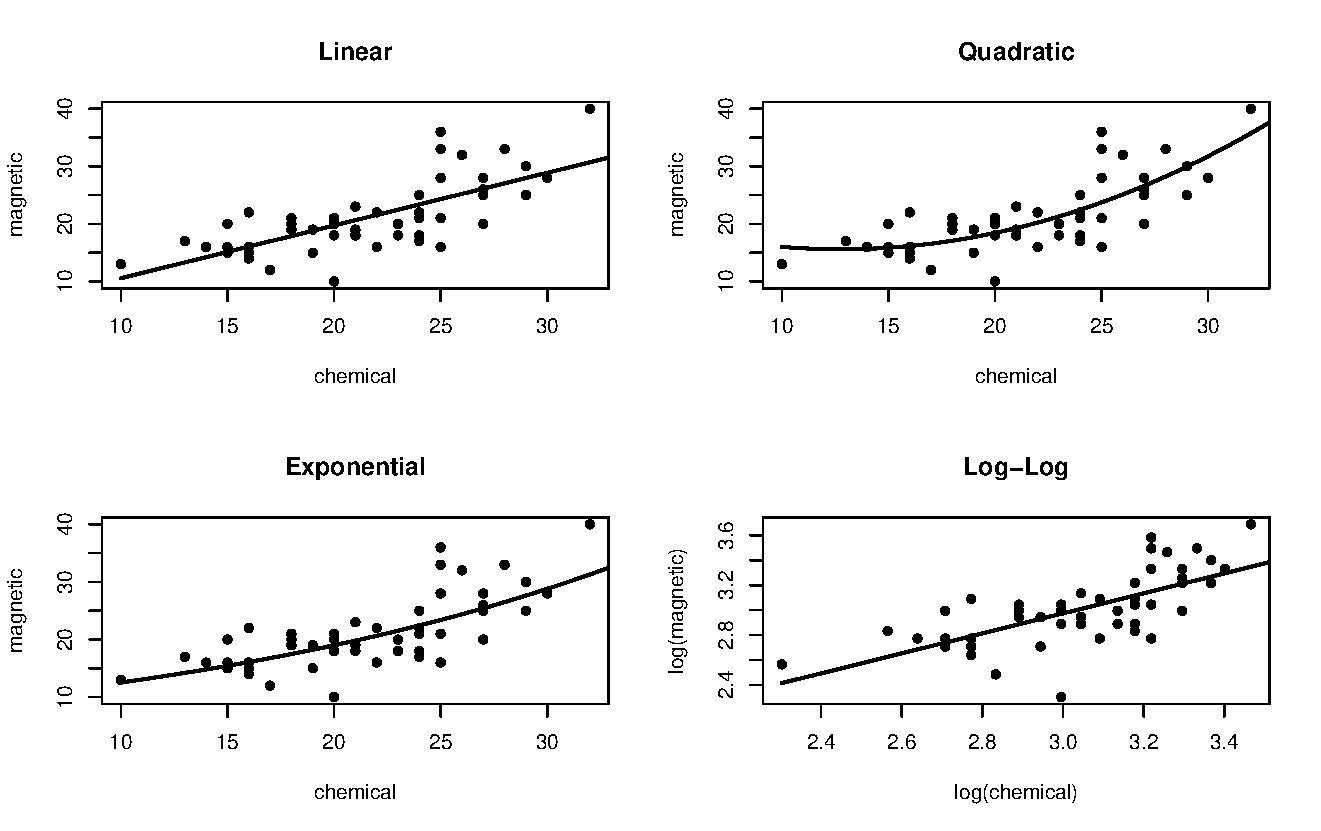
\includegraphics [width=\textwidth]{gb/K8G2}
        \caption{: Pentingnya fungsi pada Contoh 2.2: $f_{0}$, . . . ,$ f_{4}$ (baris 0:4)dengan $g(x)$ dalam $(a)$ dan rasio $g(x)/f(x)$ dalam (b).}
        \label{fig:my_label}
        \end{figure}
\end{example}
\textbf{Prosedur untuk memperkirakan kesalahan prediksi dengan n-fold (biarkan-satu-keluar) validasi silang}

\begin{enumerate}
    \item Untuk k = 1, . . . , n, biarkan pengamatan ($(x_{k},y_{k})$ menjadi titik uji dan gunakan pengamatan yang tersisa agar sesuai dengan model 
    \item Perkirakan rata-rata kesalahan prediksi kuadrat $\widehat{\sigma }_{\varepsilon }^{2}=\frac{1}{n}\sum_{k=1}^{n} e_{k}^{2}$
\end{enumerate}
\begin{example}
    (Pemilihan Model: Validasi silang). Validasi silang diterapkan untuk memilih model pada Contoh 8.16.
\begin{lstlisting}
    n <- length(magnetic) #in DAAG ironslag
e1 <- e2 <- e3 <- e4 <- numeric(n)
# for n-fold cross validation
# fit models on leave-one-out samples
for (k in 1:n) {
y <- magnetic[-k]
x <- chemical[-k]
J1 <- lm(y ~ x)
yhat1 <- J1$coef[1] + J1$coef[2] * chemical[k]
e1[k] <- magnetic[k] - yhat1
J2 <- lm(y ~ x + I(x^2))
yhat2 <- J2$coef[1] + J2$coef[2] * chemical[k] +
J2$coef[3] * chemical[k]^2
e2[k] <- magnetic[k] - yhat2
J3 <- lm(log(y) ~ x)
logyhat3 <- J3$coef[1] + J3$coef[2] * chemical[k]
yhat3 <- exp(logyhat3)
e3[k] <- magnetic[k] - yhat3
J4 <- lm(log(y) ~ log(x))
logyhat4 <- J4$coef[1] + J4$coef[2] * log(chemical[k])
yhat4 <- exp(logyhat4)
e4[k] <- magnetic[k] - yhat4
}
\end{lstlisting}
Perkiraan berikut untuk kesalahan prediksi diperoleh dari persilangan n-fold validasi.
\begin{lstlisting}
    > c(mean(e1^2), mean(e2^2), mean(e3^2), mean(e4^2))
[1] 19.55644 17.85248 18.44188 20.45424
\end{lstlisting}
Menurut kriteria kesalahan prediksi, Model 2, model kuadrat, akan menjadi yang paling cocok untuk data.
\begin{lstlisting}
    > L2
Call:
lm(formula = magnetic ~ chemical + I(chemical^2))
Coefficients:
(Intercept) chemical I(chemical^2)
24.49262 -1.39334 0.05452
\end{lstlisting}
Persamaan regresi pas untuk Model 2 adalah
\begin{equation*}
    \widehat{Y}=24.49262-1.39334X+0.05452X^{2}
\end{equation*}
Plot residual untuk Model 2 ditunjukkan pada Gambar 8.3. Cara mudah untuk dapatkan beberapa plot residual adalah dengan plot(L2). Bergantian, plot serupa bisa ditampilkan sebagai berikut
 \begin{lstlisting}
     par(mfrow = c(2, 2)) #layout for graphs
plot(L2$fit, L2$res) #residuals vs fitted values
abline(0, 0) #reference line
qqnorm(L2$res) #normal probability plot
qqline(L2$res) #reference line
par(mfrow = c(1, 1)) #restore display
 \end{lstlisting}
Bagian dari ringkasan untuk model kuadrat pas di bawah ini.
\begin{lstlisting}
    Residuals:
Min 1Q Median 3Q Max
-8.4335 -2.7006 -0.2754 2.5446 12.2665
Residual standard error: 4.098 on 50 degrees of freedom
Multiple R-Squared: 0.5931, Adjusted R-squared: 0.5768
\end{lstlisting}
Dalam model kuadrat prediktor $X dan X^{2}$ sangat berkorelasi. Melihat
poli untuk pendekatan lain dengan polinomial ortogonal.
\end{example}
\begin{figure}
    \centering
    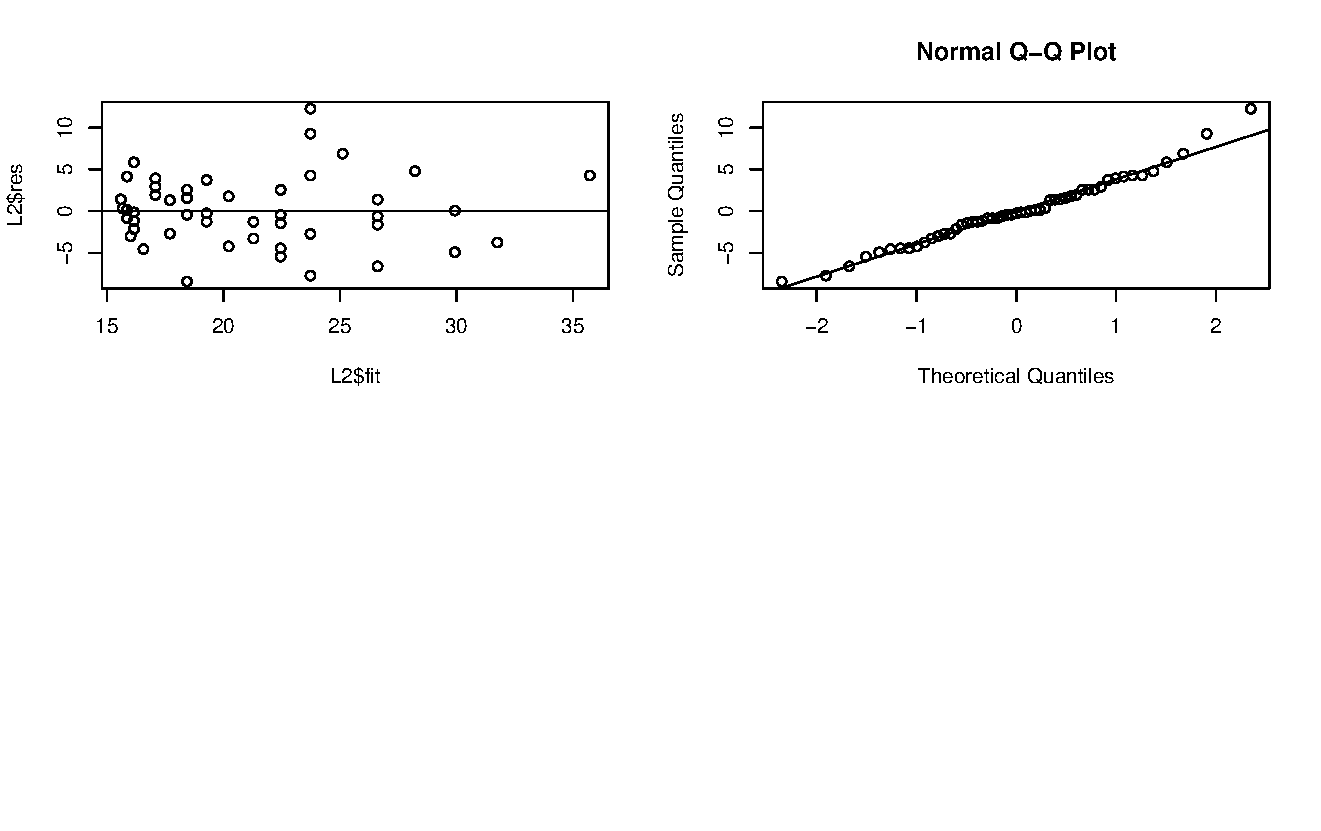
\includegraphics{gb/K8G2 (1).pdf}
    \caption{Caption}
    \label{fig:my_label}
\end{figure}
\end{document}